
% --------------------------------------------------------------------------------------
%                   LATEX TEMPLATE FOR DISSERTATION (HONS)
% --------------------------------------------------------------------------------------
\documentclass[11pt]{book}

\usepackage{amsfonts, amsmath, amssymb}  
\usepackage{times}

%\usepackage[backref=page,pagebackref=true,linkcolor = blue,citecolor = red]{hyperref}
%\usepackage[backref=page]{backref}


\usepackage{graphicx}
\DeclareGraphicsExtensions{.pdf,.png,.jpg}


\setlength{\oddsidemargin}{1.5cm}
\setlength{\evensidemargin}{0cm}
\setlength{\topmargin}{1mm}
\setlength{\headheight}{1.36cm}
\setlength{\headsep}{1.00cm}
%\setlength{\textheight}{20.84cm}
\setlength{\textheight}{19cm}
\setlength{\textwidth}{14.5cm}
\setlength{\marginparsep}{1mm}
\setlength{\marginparwidth}{3cm}
\setlength{\footskip}{2.36cm}



\begin{document}
\pagestyle{empty}

%: ----------------------------------------------------------------------
%:                  TITLE PAGE: name, degree,..
% ----------------------------------------------------------------------


\begin{center}

\vspace{1cm}

%%% Type the thesis title below%%%%%%%%%%%%%%%%
{\Huge         Nested sampling with peers}

\vspace{35mm} 


\includegraphics[width=2cm]{logo}

 \vspace{45mm}

%%%%%Type Your Name Below%%%%%%%%%%%%
{\Large       Feishuang Wang}

	\vspace{1ex}

School of Computer Science

The University of Auckland

	\vspace{5ex}

 %%%%%Typing Your Supervisors Name Below%%%%%%%%%%%%
Supervisor:             Dr Brendon James Brewer

	\vspace{30mm}

A dissertation  submitted in partial fulfillment of the requirements for the degree of Master of Professional Studies in Data Science OR Master of Data Science (delete one), The University of Auckland, 20XX.

\end{center}


  \newpage



%: --------------------------------------------------------------
%:                  FRONT MATTER:  abstract,..
% --------------------------------------------------------------
\chapter*{Abstract}       
\setcounter{page}{1}
\pagestyle{headings}
% \pagenumbering{roman}

\addcontentsline{toc}{chapter}{Abstract}
A nested sampling algorithm is a Bayesian approach to computing and comparing models and generating samples from posterior distributions. We introduce a general Monte Carlo method based on Nested Sampling, which name is Nested Sampling with peers, this method generates one particle above the threshold from the last iteration by querying the params from the server and updating it. We describe the new method over a test case and find that it has better accuracy than the original MCMC-based nested sampling with the same computational overhead.
 Put your abstract  here.  
 The abstract should contain a brief summary of the aim, methodologies, 
finding and conclusions of the dissertation.  The abstract should normally be fewer than 350 words.



%: --------------------------------------------------------------
%:                  END:  abstract
% --------------------------------------------------------------


%: ----------------------- contents ------------------------
\setcounter{secnumdepth}{3} % organisational level that receives a numbers
\setcounter{tocdepth}{3}    % print table of contents for level 3
\tableofcontents            % print the table of contents
% levels are: 0 - chapter, 1 - section, 2 - subsection, 3 - subsection



%: --------------------------------------------------------------
%:                  MAIN DOCUMENT SECTION
% --------------------------------------------------------------
	
\chapter{Introduction}%    \chapter{}  = level 1, top level

\section{Bayesian Analysis} 
The Bayesian Analysis problem is in fact a parameter estimation problem, 
The term \textit{parameter} means \textit{unknown quantity}, howerver in real world, we don't 
have enough information to decide a quantity, so we need Bayesian Analysis to help us.
The parameter you interested in are denoted by $\theta$, to estimate them, first of all, you need to 
model a probability distribution on the \textit{hypothesis space}, a \textit{hypothesis space} is the 
collection of possibilities, this means that you are modeling the initial assumptions, and the probability distribution
is called the \textit{prior}, it is the distribution of $\theta$. The data set is called D, 
after that we can use Bayes’ Theorem to determine the \textit{posterior distribution}:
\begin{equation}
	p(\theta|D) = \frac{p{(\theta)}p(D|\theta)}{p(D)}
\end{equation}
in the above equation, 
\begin{enumerate}
\item The posterior distribution is $p(\theta|D)$, given the data set $D$ with the conditional distribution of $\theta$.
 \item The prior distribution is $p{(\theta)}$.
 \item The likelihood is $p(D|\theta)$, it means the conditional probability of observing the data.
 \item  The denominator $p(D)$ is called marginal likelihood or evidence, it doesn't depend on the parameter $\theta$.
\end{enumerate}
 The posterior distribution is usually more constricted than the prior distribution, 
 indicating that we have gained some insights from the data and that our level of uncertainty about the parameter values has been lowered.
 See the Figure 1.1 for how we often see the updating from the prior distribution to a posterior distribution.
\subsection{Marginal Likelihood}
The marginal likelihood shows how does the model be constructed.
From probability theory we can learn that If you integrate over the posterior distribution, you must get 1 at the last. 
So we can write the marginal likelihood in the following form:
\begin{equation}
	p(D|I) = \int p(\theta|I)p(D|\theta, I)d\theta
\end{equation}
where $I$ represents the underlying assumptions and information, and the integral is N-dimensional, go through all the continuous parameter space, the $I$ is 
usually ignored and the marginal likelihood can be denoted as $Z$:
\begin{equation}
	Z = \int p(\theta)p(D|\theta)d\theta
\end{equation}
when sum the discrete parameter $\theta$, it also has the following form:
\begin{equation}
	Z = \sum p(\theta)p(D|\theta)
\end{equation}
The ratio of evidence values is always called Bayes factors, calculating the value of $Z$ 
is important for comparing different model assumptions, so the Z-value allows the results to be predicted into the future 
because the predicted model can be compared with the current model without the need for recalculation, in short, this parameter measures how well a model fits the data.
However, the standard algorithm such as Markov chain Monte Carlo (MCMC) are considered for posterior distribution, it cannot provide the evidence like Bayesian Inference,
for it only gives a collection of normalised posterior, it will be a challenge to get the evidence in Bayesian analysis.

% The main strength of LaTex is  mathematical typesetting.  

% There is a huge amount of information about LaTex on the internet.
% A helpful short manual, also included in this folder, is the file
% \verb+latex_intro.pdf+
% This document gives a lot of sample LaTex commands.  
% The file \verb+latex-howto.tex+ in this folder also contains examples of many latex commands.
\section{Nested Sampling} 

\subsection{Model Selection with Nested Sampling}
Consider two mutually exclusive model $M_1$ and $M_2$, $M_1$ has the parameter $\theta_1$ and $M_2$ has the 
parameter $\theta_2$, from previous method we discussed, we can calculate the posterior distribution of $\theta_1$ :
\begin{equation}
	p(\theta_1|D, M_1) = \frac{p(\theta_1|M_1)p(D|\theta_1, M_1)}{p(D|M_1)}
\end{equation}
Same, calculate the posterior distribution of $\theta_2$ 
\begin{equation}
	p(\theta_2|D, M_2) = \frac{p(\theta_2|M_2)p(D|\theta_2, M_2)}{p(D|M_2)}
\end{equation}
For simplicity, we often calculate the ratio of posterior distributions to compare models:
\begin{equation}
	\frac{p(M_1|D)}{p(M_2|D)} = \frac{p(M_1)}{p(M_2)} \times \frac{p(D|M_1)}{p(D|M_2)}
\end{equation}
The result of this formula is called \textit{posterior odds}, the posterior probability of M2 over M1 depends on the prior probability: is M2 more credible than M1 before considering the data? Another ratio is the ratio of likelihoods, sometimes called the Bayesian coefficient; how likely is the data for hypothetical M2 versus hypothetical M1? These possibilities are not the likelihood of a particular value of the parameter, but the likelihood of the entire model.
We have to use the marginal likelihood to make a better progress.
\subsection{Sorting}
In multiple dimensions, the direct integration calculation for the edge likelihood becomes unrealistic, we define the 
 $X$ as the model's prior mass, it can be integrated in this form:
 \begin{equation}
	X(\lambda) = \int _{L(\theta)> \lambda}\pi(\theta)d\theta
 \end{equation}
 we can write the inverse function $L(X)$, the marginal likelihood \textit{i.e.} evidence will
 be in this form:
 \begin{equation}
	 Z = \int ^{1}_{0} L(X) dX
 \end{equation}
 To get the inverse function, we can divide the prior into little particles and then sort all the particles by likelihood.
 In geometrical terms, the function $L(X)$ is monotonically diminishing, and the likelihood decreases as the value of X increases from 0 to 1, as shown in Figure 1.1.
From the figure1.1 we can find that when approaching the maximum likelihood, $X$ will keep decreasing.
 \begin{center}
	\begin{figure}
			\centering
			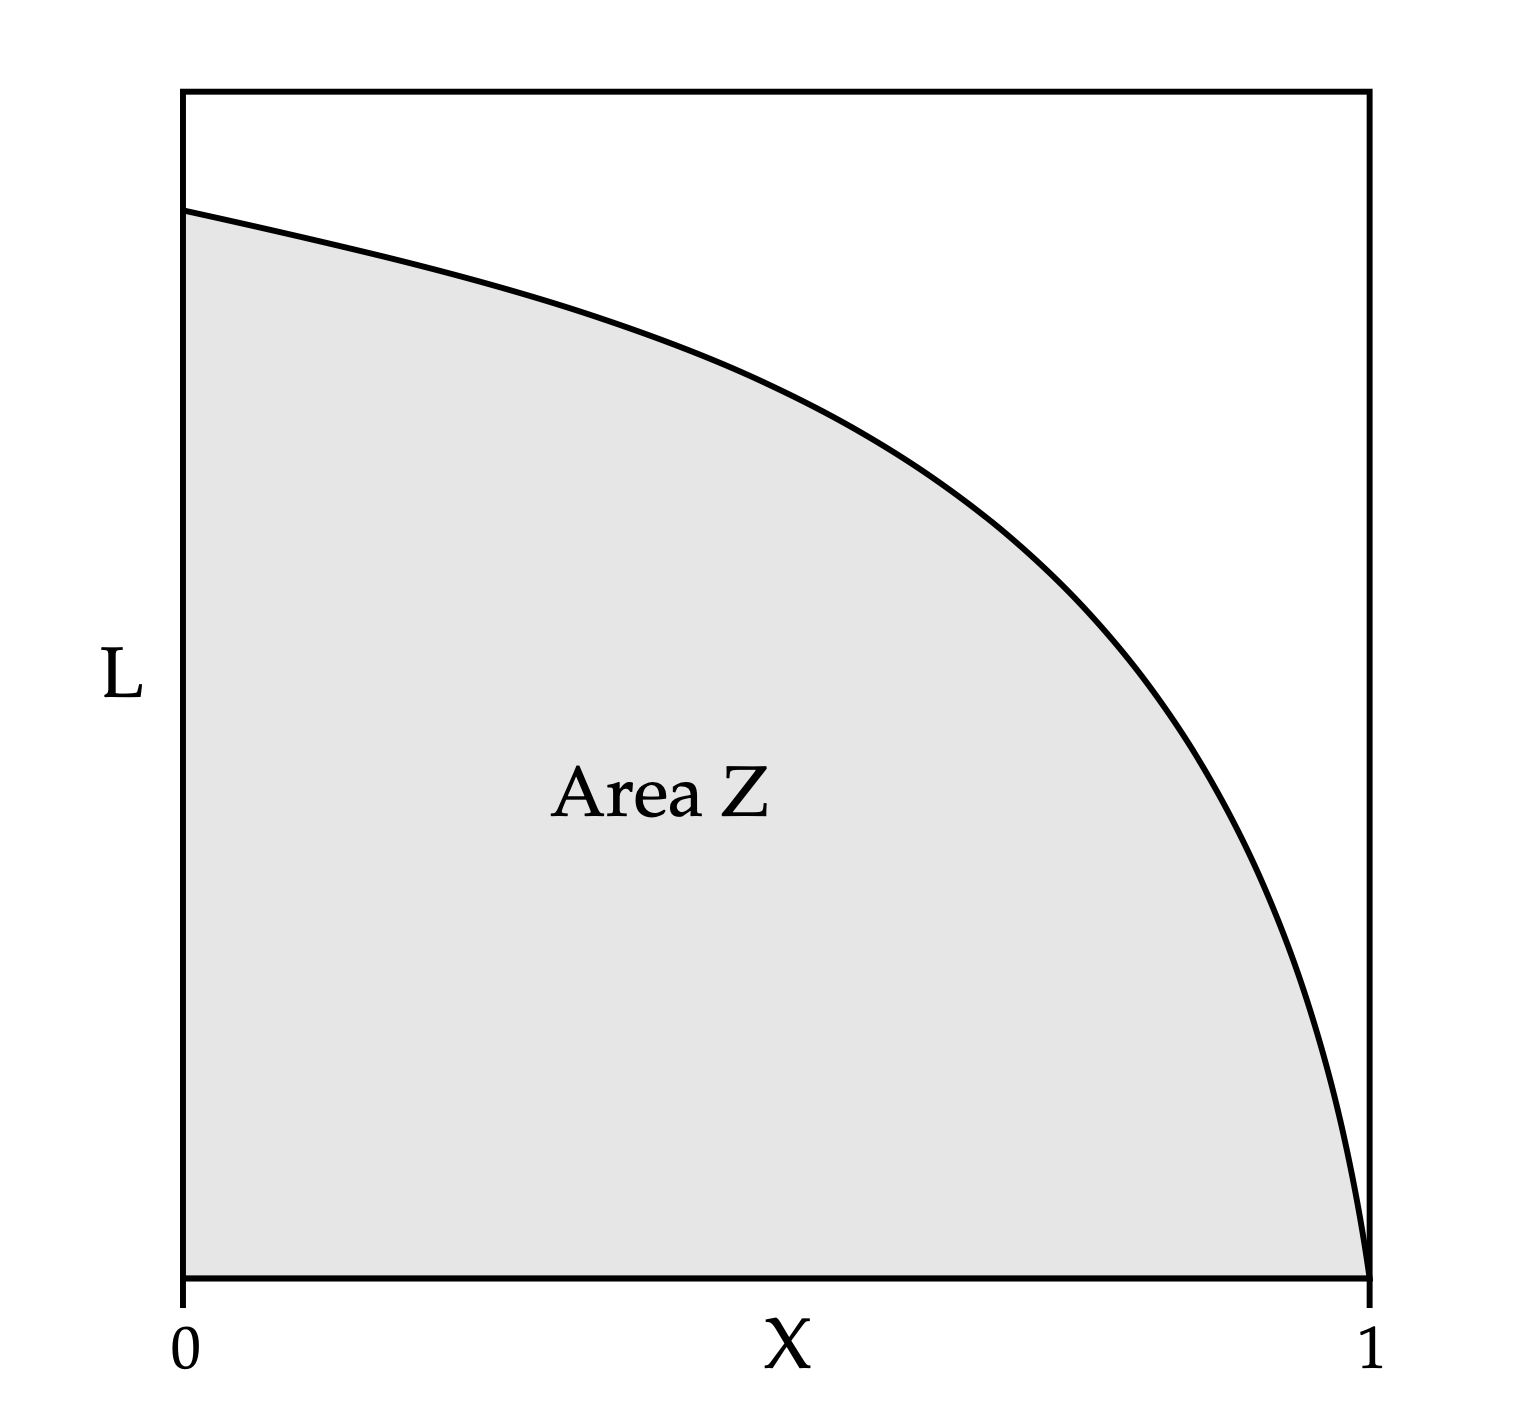
\includegraphics[width=0.6\textwidth]{areaz}
			\caption{Likelihood function with area Z.}
			\label{fig:modes}
	\end{figure}
	\end{center}

The explanation of 1.5 is that the $L(X)$ is the probability corresponding to $\lambda$ that makes the probability, $L(\theta)$, greater than $\lambda$ for $X$. 
$L(0.4) = 0.01$ may be interpreted as a 40$\%$ probability that $\pi(\theta)$ will be greater than 0.01 for $\theta$ chosen from the prior.
To evaluate the mapped integral in 1.5, Skilling proposed a simple trapezoidal rule by calculating 
weighted sums:
\begin{equation}
	Z \approx \sum_{i=1}^{j}w_iL_i (w_i = \frac{1}{2}(X_{i-1} -X_{i+1}))
\end{equation}
In every iteration i, the likelihood is $L(X_i)$, and $j$ is total number of iterations.
\subsection{A easy example}
Imagine we have a model whose parameter is a single $X$, and it the parameter $X$ follows the uniform prior distribution
$\pi(\theta)$ from 0 to 1, it also has a likelihood function $L(X)$ which is a decreasing function of X, the Figure1.2 illustrate the graph of the example,It's easy to find that in this situation, 
the evidence will be $Z = \int ^ 1 _0L(X)DX$
\begin{center}
	\begin{figure}
			\centering
			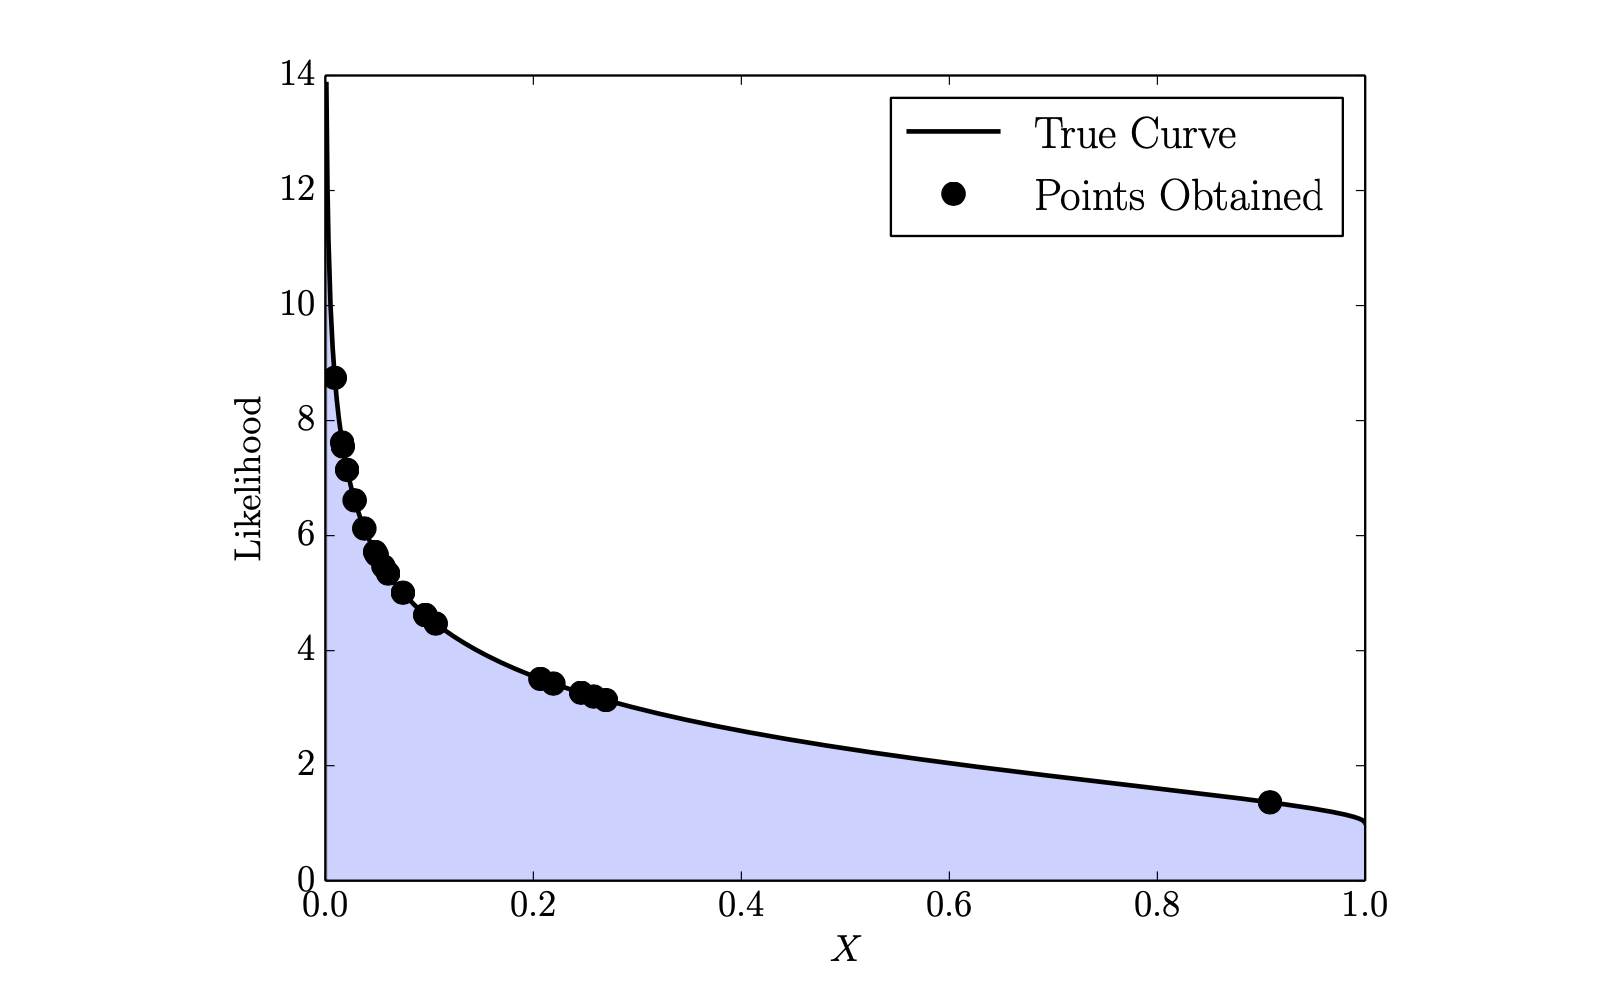
\includegraphics[width=0.6\textwidth]{example1}
			\caption{A simple model estimate problem with only one parameter}
			\label{fig:example1}
	\end{figure}
	\end{center}
\subsection{Nested Sampling Algorithms}
This section will discuss the main idea of Nested Sampling, it is a Monte Carlo algorithm and not a 
typical MCMC algorithm in technical. John Skilling proposed the algorithm specifically for approximating these marginal integrals, \textit{i.e.}, evidence, and it also generates samples from the posterior distribution. 
In the prior distribution $\pi(\theta)$, it needs to generate $N$ \textit{particles or live points} $\theta$, just like an vector to initialize the starting state.
To approximating the evidence, there's some important steps, if we find the points with the worst likelihood,
always denoted by $L_{worst}$ and this is often associated with the highest $X$ value, If different particle $N$ are taken, 
the highest $X$ value will always be close to $X = 1$ and not close to $X = 0$. 
Skilling (2006) gives a simple treatment by estimating $X_{worst} = e^{(\frac{-1}{N})}$, 
and we also know the probability of this point.By generating a new point from 
the prior distribution to replace the worst $X_{worst}$, more points can be obtained, 
and the restriction is that the likelihood of the point must be higher than $L_{worst}$.
And in the second iteration, the estimation of the X value who has a worst particle is $e^{(\frac{-1}{N})} \times e^{(\frac{-1}{N})} = e^{(\frac{-2}{N})}$,
Because we already know the likelihood, so we can contine the iteration.


\section{Distributed System}
\subsection{BONIC}
\section{Spakslab Problem}

\chapter{Implementation}
We first show  some simple examples of 
mathematical formulae using latex typesetting.

\begin{enumerate}
\item The basic functions: $\cos(x),  \sin(x),   \ln(x) $,  (\verb+$\cos(x),\sin(x),\ln(x)$+). 
\item Greek letters: $\alpha \beta \gamma \delta\epsilon...$ (\verb+$\alpha\beta\gamma\delta\epsilon...$+).
\item Mathematical symbols: $\int  \oint \sum\lim\bigcup \bigcap$
 (\verb+$\int\oint\sum\lim\bigcup\bigcap$+).
\item Fractions: $\frac{1}{2},\frac{1}{2-x}$ (\verb+$\frac{1}{2},\frac{1}{2-x}$+).
\end{enumerate}

The following matrix 
\begin{eqnarray}\label{eqn:matrix}
\left[
\begin{array}{ccc}
	 U_{r}&     r       &   W_{r}	\\
	   0       &	1      &  V_{x}	\\
	   0	   &	0      &  W_{x}
\end{array}
\right], 
\end{eqnarray}
is generated using  the \verb+equarray+ environment:
\begin{verbatim}
\begin{eqnarray}\label{eqn:matrix}
\left[
\begin{array}{ccc}
	 U_{r}& r &W_{r}\\
	   0 &1 &V_{x}\\
	   0&	0 & W_{x}
\end{array}
\right], 
\end{eqnarray}
\end{verbatim}
The \verb+\label{eqn:matrix}+ command labels the equation with \verb+{eqn:matrix}+ which can 
be referred  to somewhere else in the text by using \verb+\ref{eqn:matrix}+ or  \verb+\eqref{eqn:matrix}+.


The command \verb+\notag+ eliminates the numbering of the first equation,
\begin{eqnarray} \label{eqn:lambda_trace}
\lambda^{(1)}&=&tr[T^{(1)}P],\notag  \\
\lambda^{(2)}&=&tr[T^{(2)}P - T^{(1)}ST^{(1)}P].
\end{eqnarray}
\begin{verbatim}
\begin{eqnarray} \label{eqn:lambda_trace}
\lambda^{(1)}&=&tr[T^{(1)}P],\notag  \\
\lambda^{(2)}&=&tr[T^{(2)}P - T^{(1)}ST^{(1)}P].
\end{eqnarray}
\end{verbatim}


\subsection{Itemized lists}
Example of an itemized list:
\begin{itemize}
\item muscle and fat cells remove glucose from the blood,
\item cells use glucose for protein synthesis.
\end{itemize}
\begin{verbatim}
\begin{itemize}
\item muscle and fat cells remove glucose from the blood,
\item cells use glucose for protein synthesis.
\end{itemize}
\end{verbatim}
This can be done by an enumerated  list:
\begin{enumerate}
\item muscle and fat cells remove glucose from the blood,
\item cells use glucose for protein synthesis.
\end{enumerate}

\begin{verbatim}
\begin{enumerate}
\item muscle and fat cells remove glucose from the blood,
\item cells use glucose for protein synthesis.
\end{enumerate}
\end{verbatim}



\newpage



\subsection{Inserting figures}


You may save your Matlab figures as jpg files.  Figures should  be stored in the 
same folder as the latex files.
For the graphicx package to work you usually need to ask latex to create a pdf file (e.g., command pdflatex or latexpdf).

An example of an inserted image is given in Figure~\ref{fig:modes}.

\begin{center}
\begin{figure}[h]
		\centering
		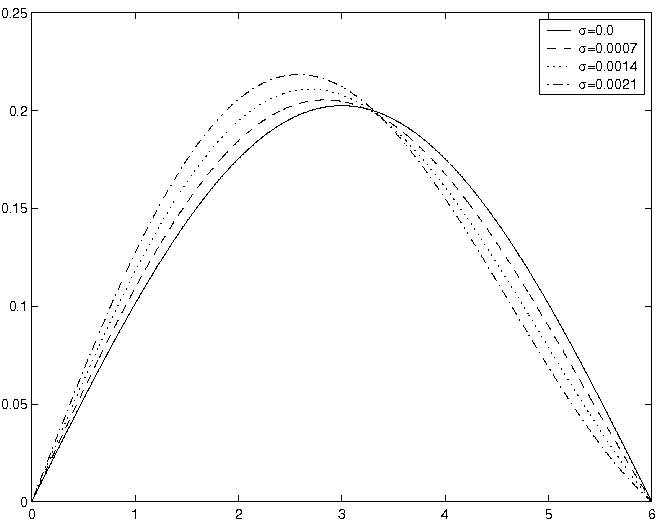
\includegraphics[width=0.6\textwidth]{modes}
		\caption{Mode shapes}
		\label{fig:modes}
\end{figure}
\end{center}




 
\subsection{Tables}\label{table}
Example of a table,
\begin{table}[htp]
\centering
\begin{tabular}{ccc} % ccc means 3 columns, all centered; alternatives are l, r
{\bf Gene} & {\bf GeneID} & {\bf Length} \\ 
\hline % draws a line under the column headers
human latexin & 1234 & 14.9 kbps \\
mouse latexin & 2345 & 10.1 kbps \\
rat latexin   & 3456 & 9.6 kbps \\
\end{tabular}
\caption[title of table]{\textbf{title of table} - Overview of latexin genes.}
\label{latexin_genes} % label for cross-links with \ref{latexin_genes}
\end{table}
\begin{verbatim}
\begin{table}[htp]
\centering
\begin{tabular}{ccc} 
% ccc means 3 columns, all centered; alternatives are l, r
{\bf Gene} & {\bf GeneID} & {\bf Length} \\ 
\hline % draws a line under the column headers
human latexin & 1234 & 14.9 kbps \\
mouse latexin & 2345 & 10.1 kbps \\
rat latexin   & 3456 & 9.6 kbps \\
\end{tabular}
\caption[title of table]{\textbf{title of table} - Overview of latexin genes.}
\label{latexin_genes} % label for cross-links with \ref{latexin_genes}
\end{table}
\end{verbatim}
See how to add two vertical lines in the table (Simply change \verb+{ccc}+ to \verb+{c|c|c}+)
\begin{table}[htp]
\centering
\begin{tabular}{c|c|c} % ccc means 3 columns, all centered; alternatives are l, r
{\bf Gene} & {\bf GeneID} & {\bf Length} \\ 
\hline % draws a line under the column headers
human latexin & 1234 & 14.9 kbps \\
mouse latexin & 2345 & 10.1 kbps \\
rat latexin   & 3456 & 9.6 kbps \\
\end{tabular}
\caption[title of table]{\textbf{title of table} - Overview of latexin genes.}
\label{latexin_genes2} % label for cross-links with \ref{latexin_genes}
\end{table}





\subsection{How to Refer to Equations, Sections, etc}%    \subsection{}    = level 3
 \begin{enumerate}
 \item References can be linked to equations, figures, tables or sections using the command 
 \verb+\ref+:
 Equation (\ref{eqn:lambda_trace}),  Figure~\ref{fig:modes},  Table~\ref{latexin_genes2} and Section~\ref{table}.\\
\verb+Equation~(\ref{eqn:lambda_trace}),Figure~\ref{modes},+\\
\verb+Table~\ref{latexin_genes2} and Section~\ref{table}.+


\item 
Equations can be conveniently  referred to using \verb+ \eqref+. See, for example,  Equation \eqref{eqn:lambda_trace}. \\
\verb+Equation \eqref{eqn:lambda_trace}+\\
Note that \verb+\eqref+ includes the round brackets by itself. 

\item  Citations are in a similar way but using the command \verb+\cite+:

  \cite{Salmond}, \cite{Stull}, and \cite{TandC}, 
   or  \cite{Salmond,Stull,TandC} .
   
  \begin{verbatim}   
   \cite{Salmond}, \cite{Stull}, and \cite{TandC}, 
   or  \cite{Salmond,Stull,TandC} .
 \end{verbatim} 

There are many different styles for writing citations -- you should follow the norms for your subject area.

A more advanced way to do citations is to use \verb+bibtex+.  This is a powerful tool and we encourage you to try it.  There is plenty of information about it on the web.

 
 \end{enumerate}
 
 
 
\chapter{Methodologies and analysis}
\section{Methodologies}
\section{Analysis}
\chapter{Discussion }
\section{Main results}
\section{Discussion}
\chapter{Conclusions}
You may add more chapters as needed in the file.

% --------------------------------------------------------------

% --------------------------------------------------------------
\renewcommand{\bibname}{References} % changes the header; default: Bibliography
\begin{thebibliography}{99} 
\addcontentsline{toc}{chapter}{References}


\bibitem{Farge} Farge Marie, {\em Wavelet Transforms and Their Applications to Turbulence},  \\Ann. Rev. Fluid Mech. volume 24, pages 395-457, 1992.
%ref. for an article
\bibitem{Salmond}  Salmond Jennifer,  {\em Vertical Mixing of Ozone in the Very Stable Nocturnal Boundary Layer}, PhD Thesis, University of British Columbia, 2001.
%ref. for a Thesis.
\bibitem{Stull} Stull B. Ronald, {\em Introduction to Boundary Layer Meteorology}, Dordrecht; Boston: Kulwer Academic Publishers, 1988. %%%ref. for a book
\bibitem{TandC} Torrence Christopher, Compo Gilbert P., {\em A Practical Guide to Wavelet Analysis}, Bulletin of the American Meteorological Society volume 79, pages 61-78, 1998. 
%ref. for an article
\end{thebibliography}


\appendix%%% start appendices here 
\chapter{Some extra things} 

This is an optional chapter for any additional material that does not fit 
conveniently into the body of the text (e.g., data, copies of computer programmes). 
Note that appendices won't necessarily be marked.


\end{document}
